\chapter{Auswertung}
\label{sec: Hauptkapitel 3}
Um das Volumen der Tasse möglichst genau zu bestimmen, wird zunächst das Gewicht der leeren Tasse und das Gewicht der bis zum Rand 
mit Wasser gefüllten Tasse bestimmt. 
In Excel wird das Gewicht der leeren Tasse vom Gesamtgewicht abgezogen, so dass mit der bekannten Dichte des Wassers das 
Volumen der Tasse nach der Formel \ref{eq: Tassenvolumen} berechnet werden kann.
\\

\begin{equation}
    V_{\text{Tasse}} = \frac{m_{\text{Wasser}}}{\rho_{\text{Wasser}}}
    \label{eq: Tassenvolumen}
\end{equation}


\noindent
Nach der Bestimmung des Tassenvolumens beginnen die Messungen, bei denen verschiedene Zustände und deren Kombinationen untersucht 
werden. 
Dabei werden im Wesentlichen drei Faktoren berücksichtigt: Erstens die Korngröße, wobei Kaffeepulver und Kaffeebohnen miteinander 
verglichen werden. 
Zweitens die Feuchtigkeit, wobei zwischen trockenem und feuchtem Zustand ($20\%$ Wassergehalt) unterschieden wird. 
Drittens die Verunreinigung, wobei jeweils $20\%$ des einen Materials (entweder Kaffeepulver oder Kaffeebohnen) dem anderen 
Material zugesetzt werden. 
Für jeden Zustand werden drei Messungen durchgeführt.
\\


\noindent
Bei jeder Messung wird die Schüttdichte bestimmt. Anschließend wird der Mittelwert und die Standardabweichung der Schüttdichten 
berechnet.
Der nächste Schritt ist die Berechnung der Normalverteilungen für die verschiedenen Zustände und der Vergleich der 
Normalverteilungen untereinander in Form von Diagrammen.
%==============================================================================================

\section{Kaffeebohne trocken - Kaffeepulver trocken}
    % Bild Kaffeebohne trocken -Kaffeepulver trocken
    \begin{figure}[H]
        \centering
        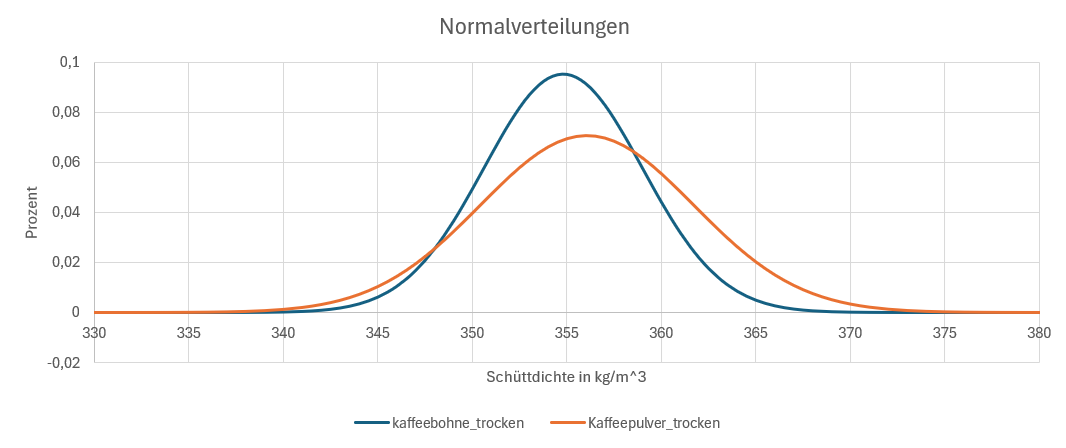
\includegraphics[width=0.8\textwidth]{Kaffeebohnen-Kaffeepulver-trocken.png}
        \caption{Normalverteilung Kaffeebohne-Kaffeepulver-trocken}
        \label{fig: Norm.trocken}
    \end{figure}

    Abbildung \ref{fig: Norm.trocken} zeigt die Normalverteilungen der Schüttdichte der Messungen von Kaffeebohnen und 
    Kaffeepulver in trockenem Zustand. 
    Die beiden Verteilungen überlappen sich deutlich, was darauf hinweist, dass es keine signifikanten Unterschiede in 
    der Schüttdichte zwischen Kaffeepulver und Kaffeebohnen im trockenen Zustand gibt.
%==============================================================================================

% 2.Auswertung
\section{Kaffeebohne trocken - Kaffeebohne feucht}
 % Bild Kaffeebohne trocken -Kaffeepulver trocken
 \begin{figure}[H]
    \centering
    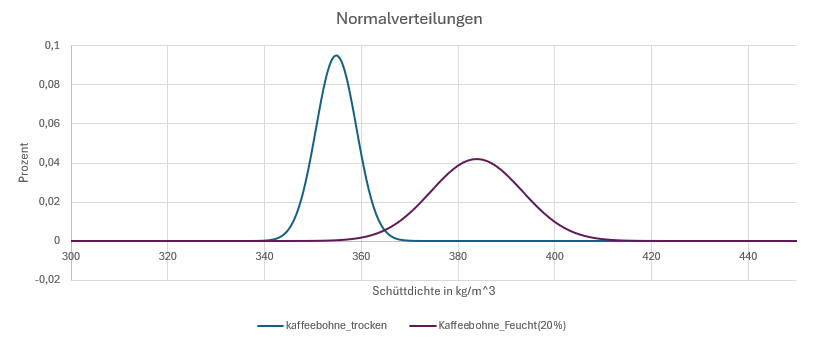
\includegraphics[width=0.8\textwidth]{Kaffeebohnen-trocken-feucht.png}
    \caption{Normalverteilung Kaffeebohne-Trocken vs Feucht}
    \label{fig: Norm.Kaffeebohne-trocken-feucht}
\end{figure}

Abbildung \ref{fig: Norm.Kaffeebohne-trocken-feucht} zeigt die Normalverteilungen der Schüttdichte der Messungen von trockenen 
Kaffeebohnen im Vergleich zu feuchten Kaffeebohnen. 
Die beiden Verteilungen überlappen sich kaum, sodass man schlussfolgern kann, dass die Schüttdichte der feuchten 
Kaffeebohnen signifikant höher ist als die der trockenen Kaffeebohnen.
%==============================================================================================

\section{Kaffeepulver trocken - Kaffeepulver feucht}
 % Bild Kaffeebohne trocken -Kaffeepulver trocken
 \begin{figure}[H]
    \centering
    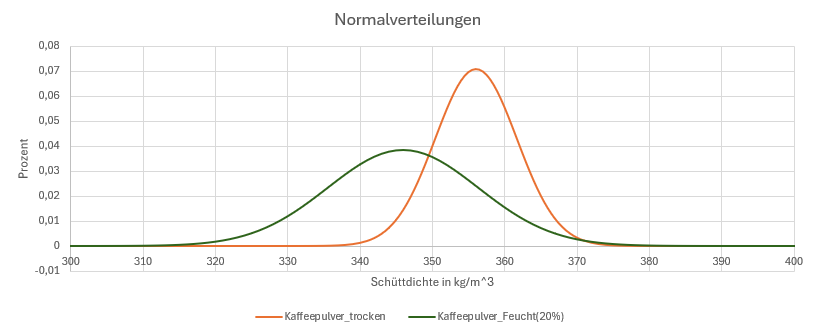
\includegraphics[width=0.8\textwidth]{Kaffeepulver-trocken-feucht.png}
    \caption{Normalverteilung Kaffeepulver-Trocken vs Feucht}
    \label{fig: Norm.Kaffeepulver-trocken-feucht}
\end{figure}

Abbildung \ref{fig: Norm.Kaffeepulver-trocken-feucht} zeigt die Normalverteilungen der Schüttdichte der Messungen von trockenem 
Kaffeepulver im Vergleich zu feuchtem Kaffeepulver. 
Die beiden Verteilungen überlappen sich zu ca. $50\%$, was darauf hinweist, dass es höchstwahrscheinlich keine signifikanten 
Unterschiede in der Schüttdichte gibt. Um die Aussage abzusichern sind weitere Messungen erforderlich.
%==============================================================================================

\section{Kaffeebohne feucht - Kaffeepulver feucht}
 % Bild Kaffeebohne trocken -Kaffeepulver trocken
 \begin{figure}[H]
    \centering
    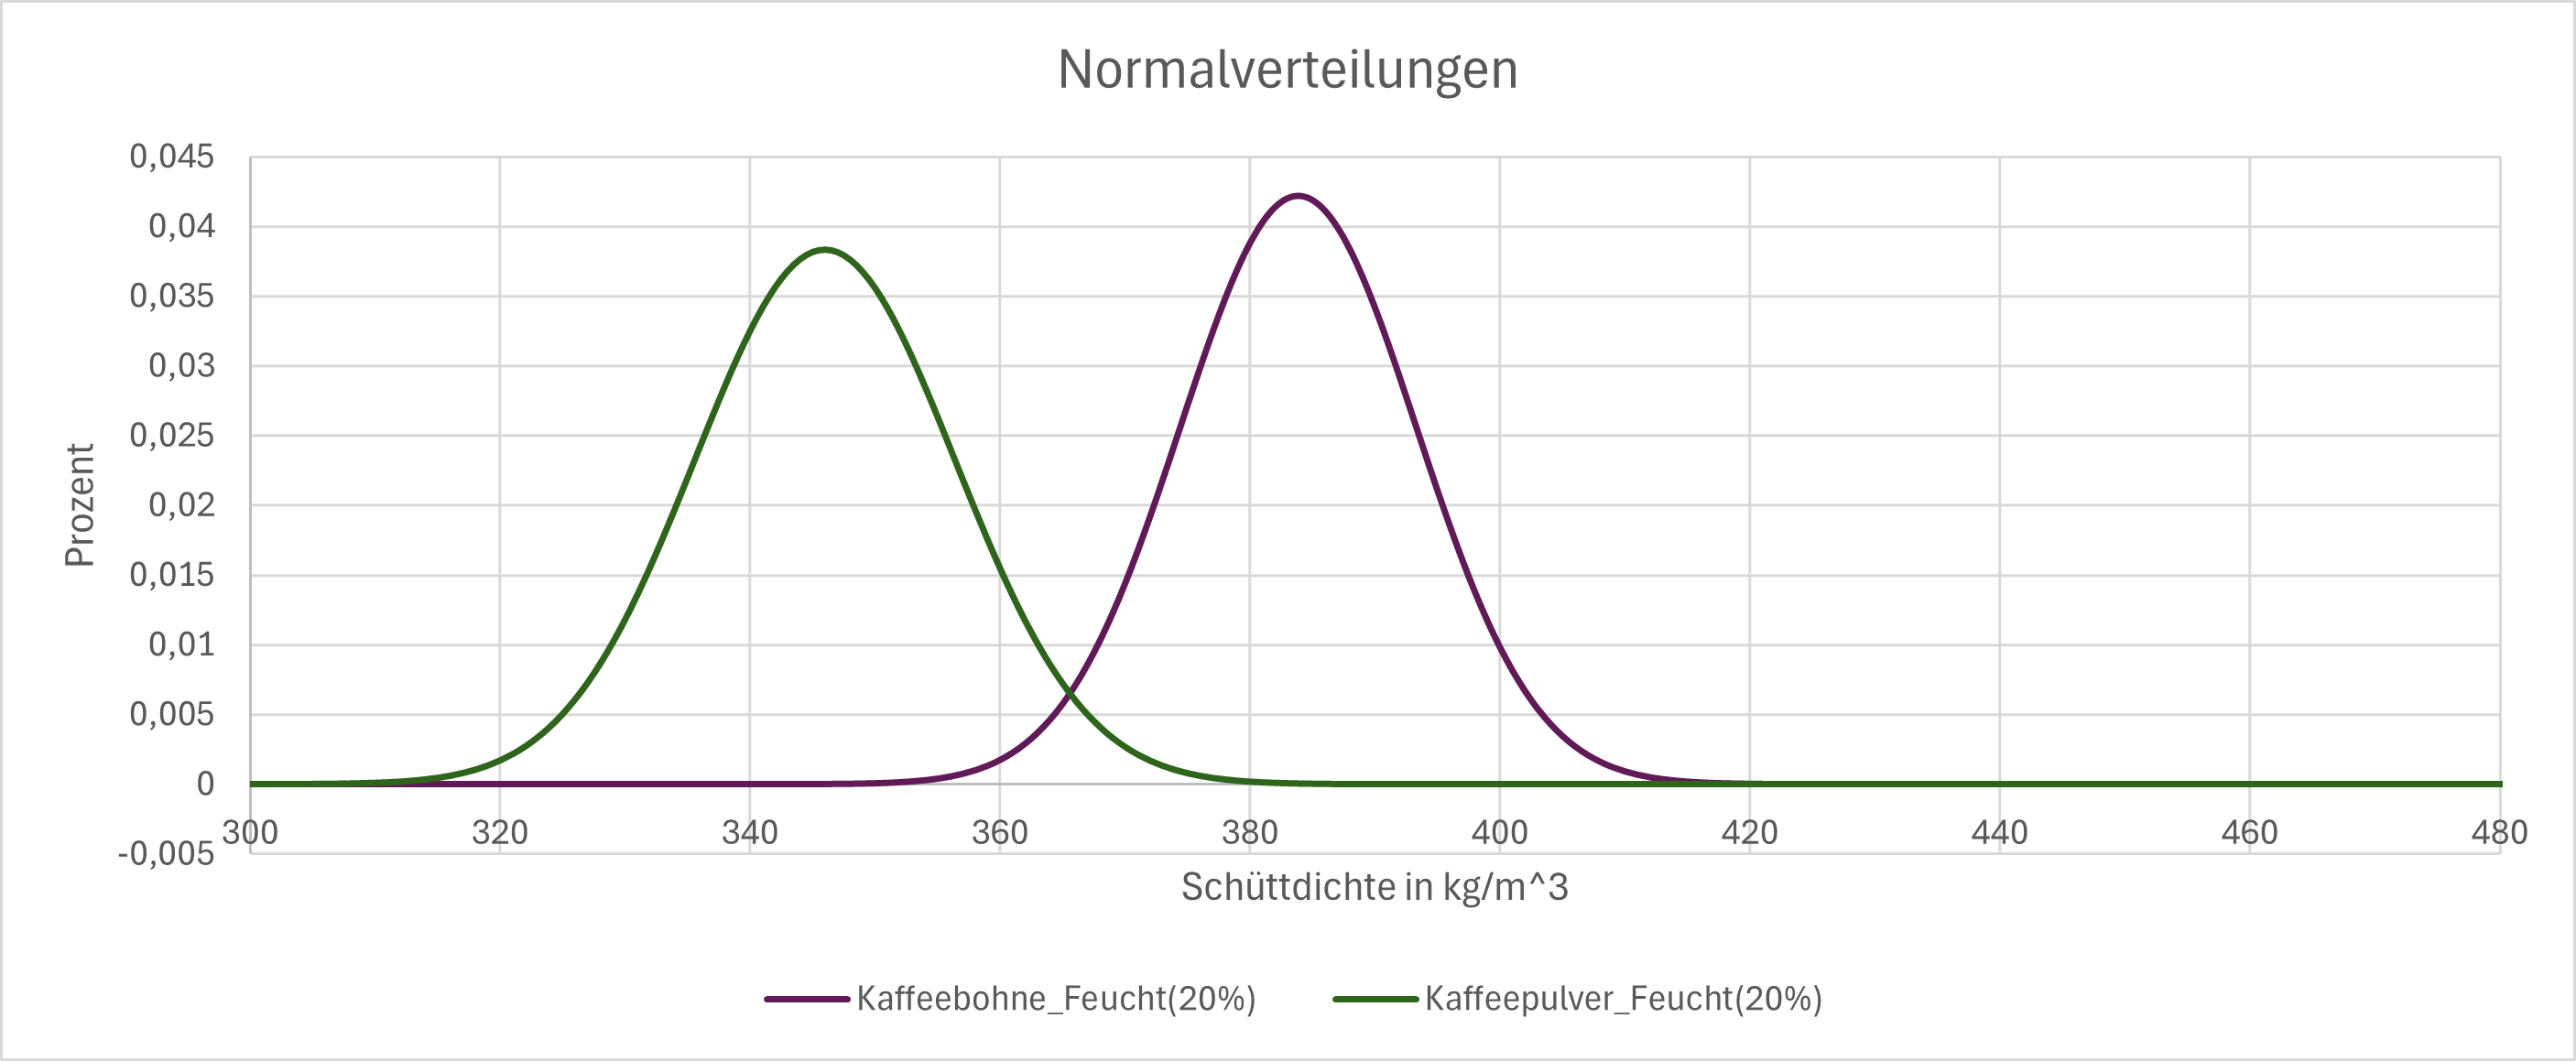
\includegraphics[width=0.8\textwidth]{Kaffeebohne_feucht-Kaffeepulver_feucht.png}
    \caption{Normalverteilung Kaffeebohne feucht vs Kaffeepulver feucht}
    \label{fig: Norm.Kaffeebohne_feucht-Kaffeepulver_feucht}
\end{figure}

Abbildung \ref{fig: Norm.Kaffeebohne_feucht-Kaffeepulver_feucht} stellt die Schüttdichte von feuchten Kaffeebohnen und feuchtem Kaffeepulver mit einem Feuchtegehalt von jeweils $20\%$ gegenüber.
Die beiden Normalverteilungen überlappen sich nur geringfügig, wobei das feuchte Kaffeepulver einen höheren 
Mittelwert der Schüttdichte aufweist als die Kaffeebohnen. Dies verdeutlicht, dass die Korngröße einen entscheidenden 
Einfluss auf die Schüttdichte hat.
%==============================================================================================

\section{Kaffepulver trocken - Verunreinigtes Kaffeepulver trocken}
 % Bild Kaffeebohne trocken -Kaffeepulver trocken
 \begin{figure}[H]
    \centering
    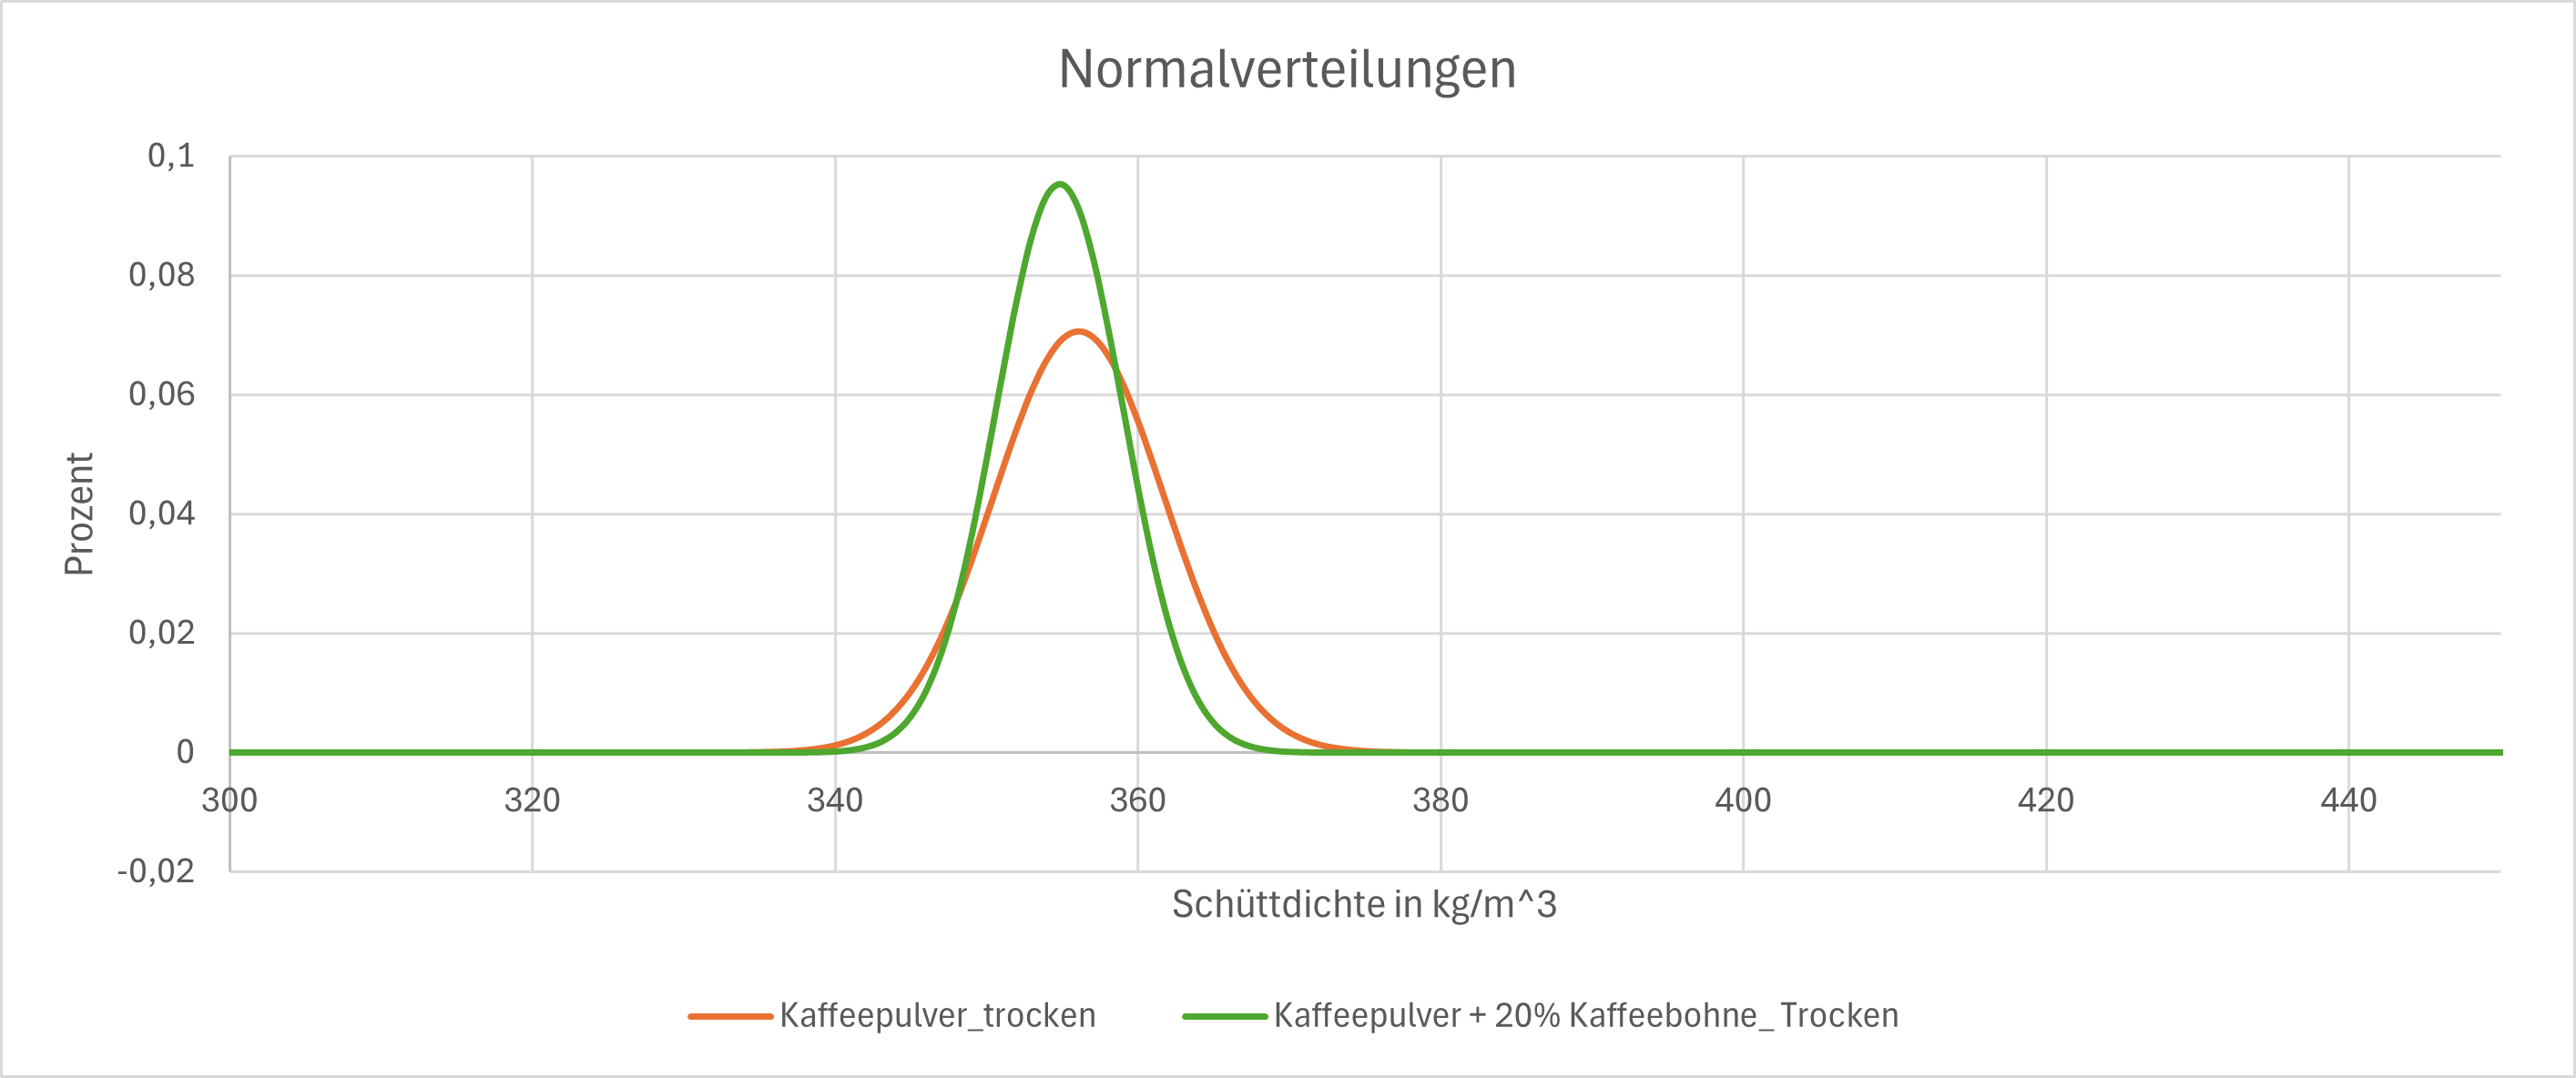
\includegraphics[width=0.8\textwidth]{Kaffeepulver-verunreinigung-trocken.png}
    \caption{Normalverteilung Kaffeepulver-Verunreinigung-trocken}
    \label{fig: Norm.Kaffeepulver-verunreinigung-trocken}
\end{figure}

Abbildung \ref{fig: Norm.Kaffeepulver-verunreinigung-trocken} zeigt die Normalverteilungen der Schüttdichte von trockenem Kaffeepulver und von Kaffeepulver, 
das mit $20\%$ trockenen Kaffeebohnen verunreinigt ist. Die Verteilungen sind nahezu identisch. Dies deutet darauf hin, 
dass die Verunreinigung des Kaffeepulvers keinen signifikanten Einfluss auf die Schüttdichte hat.
%==============================================================================================

\section{Kaffeebohne trocken - Verunreinigte Kaffeebohne trocken}
 % Bild Kaffeebohne trocken -Kaffeepulver trocken
 \begin{figure}[H]
    \centering
    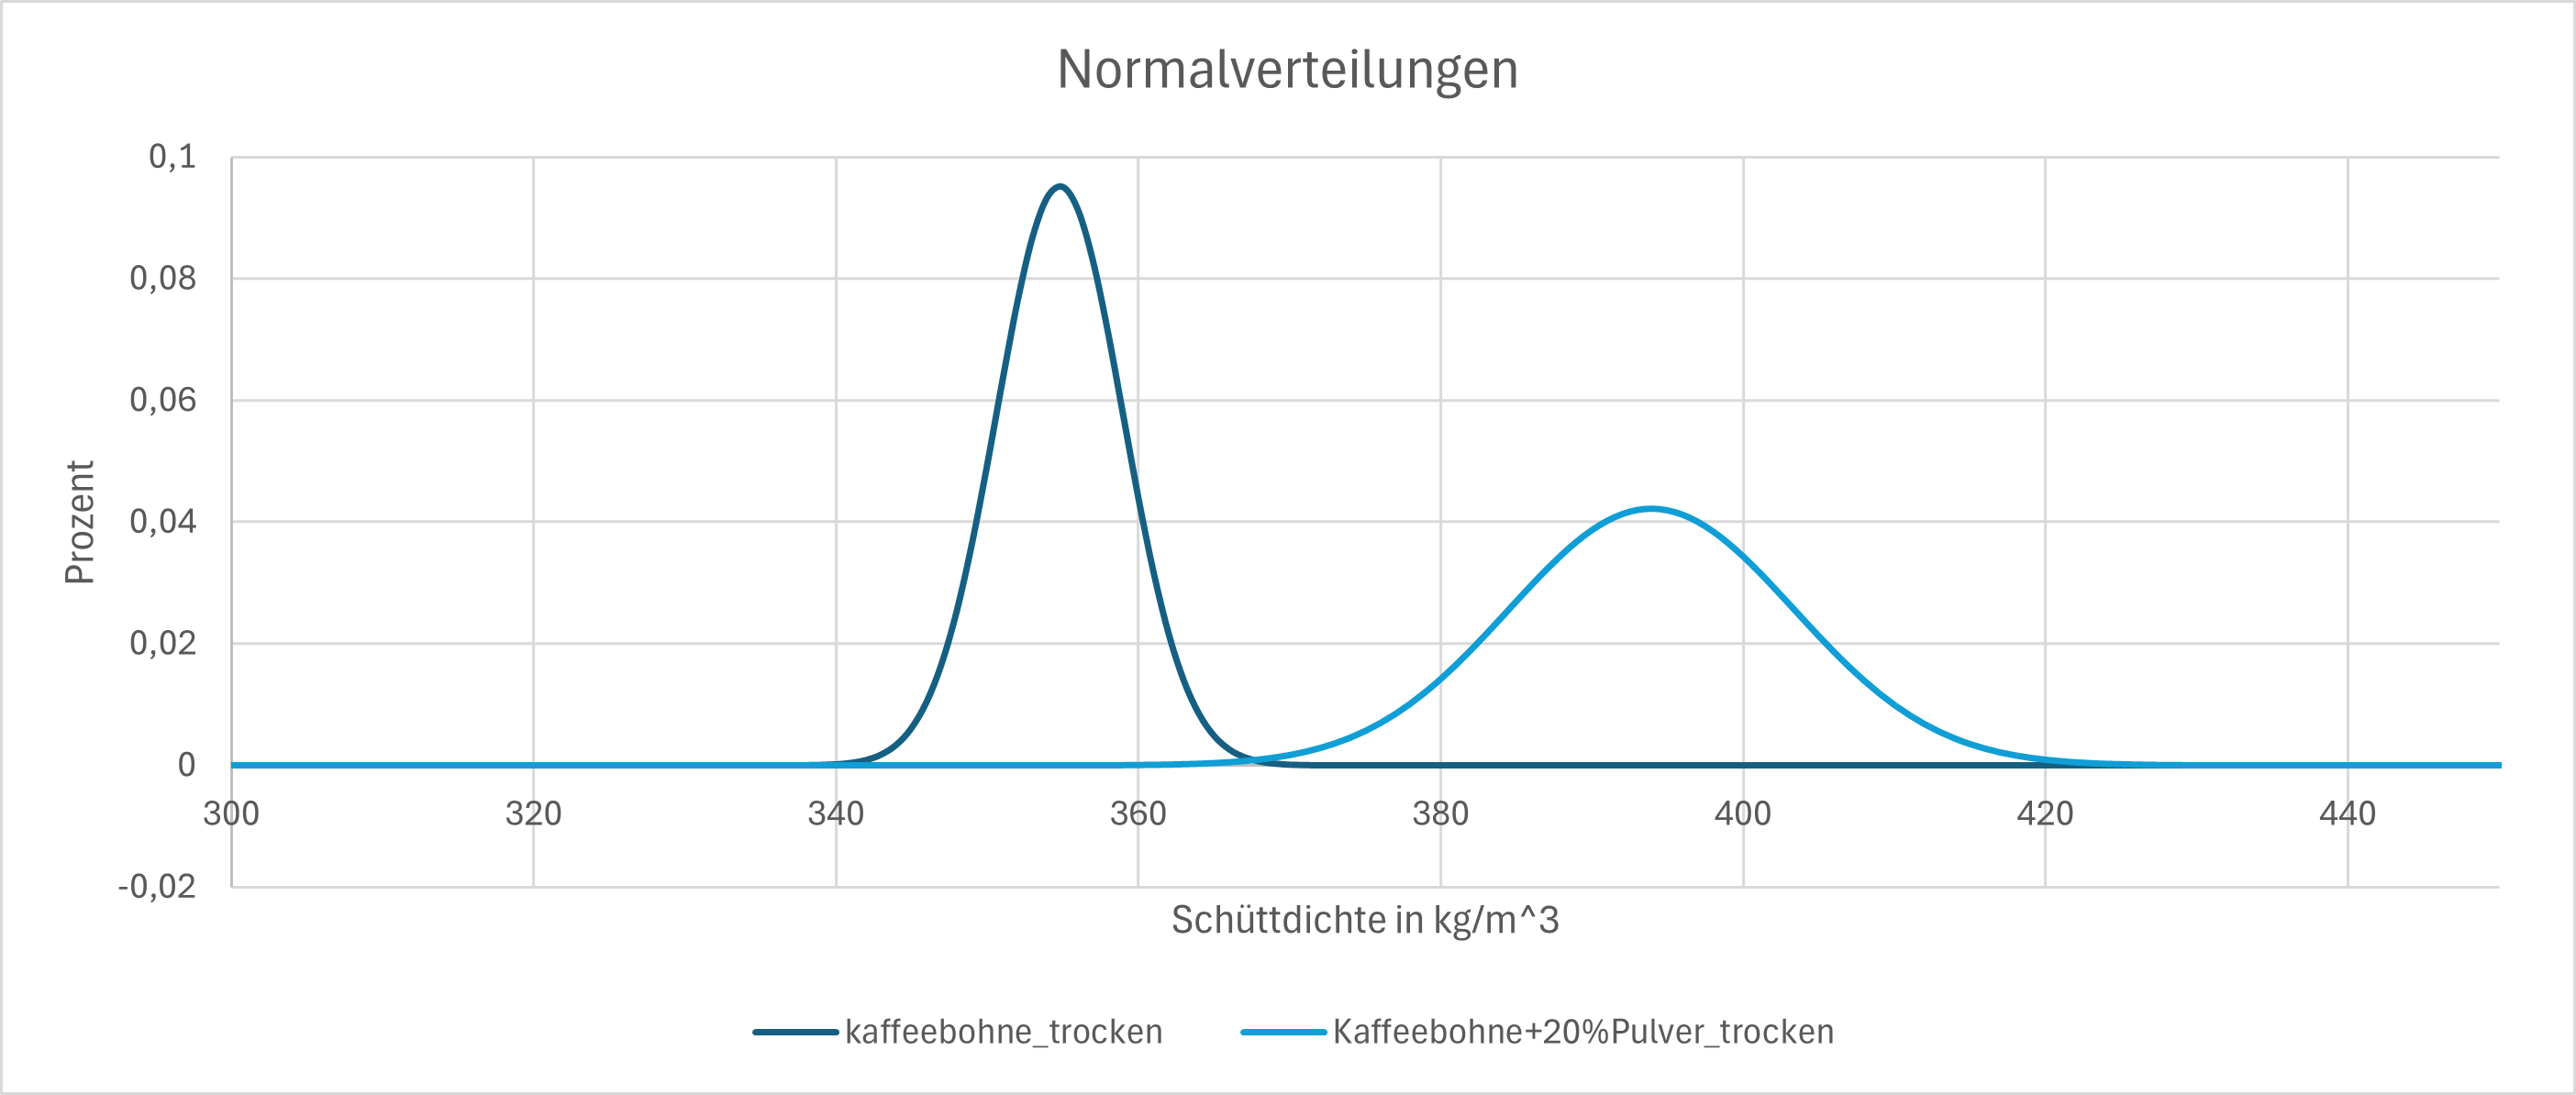
\includegraphics[width=0.8\textwidth]{Kaffeebohne-verunreinigung-trocken.png}
    \caption{Normalverteilung Kaffeebohne-Verunreinigung-trocken}
    \label{fig: Norm.Kaffeebohne-verunreinigung-trocken}
\end{figure}

Aus Abbildung \ref{fig: Norm.Kaffeebohne-verunreinigung-trocken}, in welcher die Schüttgutdichte von trockenen Kaffeebohnen mit
trockenen, verunreinigten Bohnen verglichen wird, lässt sich eine signifikant höhere Schüttgutdichte auf Seite der verunreinigten
Kaffebohnen erkennen.
%==============================================================================================

\section{Verunreinigte Kaffeebohne trocken - Verunreinigtes Kaffepulver trocken}
 % Bild Kaffeebohne trocken -Kaffeepulver trocken
 \begin{figure}[H]
    \centering
    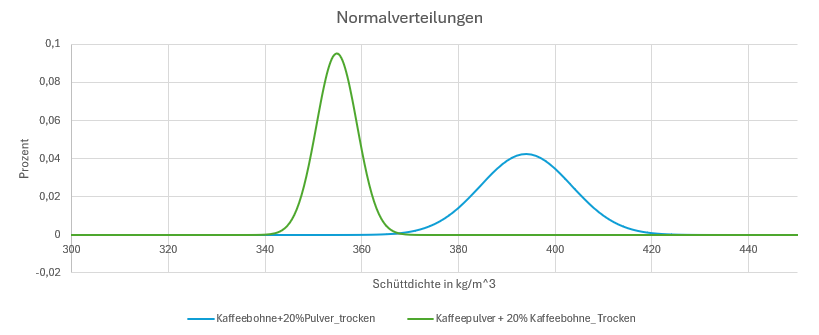
\includegraphics[width=0.8\textwidth]{Verunreinigung-trocken.png}
    \caption{Normalverteilung Verunreinigung-trocken}
    \label{fig: Norm.Verunreinigung-trocken}
\end{figure}

Abbildung \ref{fig: Norm.Verunreinigung-trocken} zeigt die Normalverteilungen der Schüttdichte für die Messungen im trockenen Zustand, bei denen jeweils eine Verunreinigung von $20\%$ vorgenommen wurde: 
einmal durch Zugabe von $20\%$ Kaffeepulver zu den Kaffeebohnen und einmal durch Zugabe von $20\%$ Kaffeebohnen zu dem Kaffeepulver. 
Im Diagramm ist deutlich zu erkennen, dass die Mischung aus Kaffeebohnen mit $20\%$ Kaffeepulver eine signifikant höhere Schüttdichte 
aufweist als die umgekehrte Kombination. 
Die nahezu fehlende Überlappung der Verteilungen bestätigt den signifikanten Unterschied in der Schüttdichte zwischen den beiden 
Mischungen.
%==============================================================================================

\section{Verunreinigung Kaffeebohne trocken vs feucht}
    % Bild Kaffeebohne trocken -Kaffeepulver trocken
    %-----------------------------------------------
    \begin{figure}[H]
        \centering
        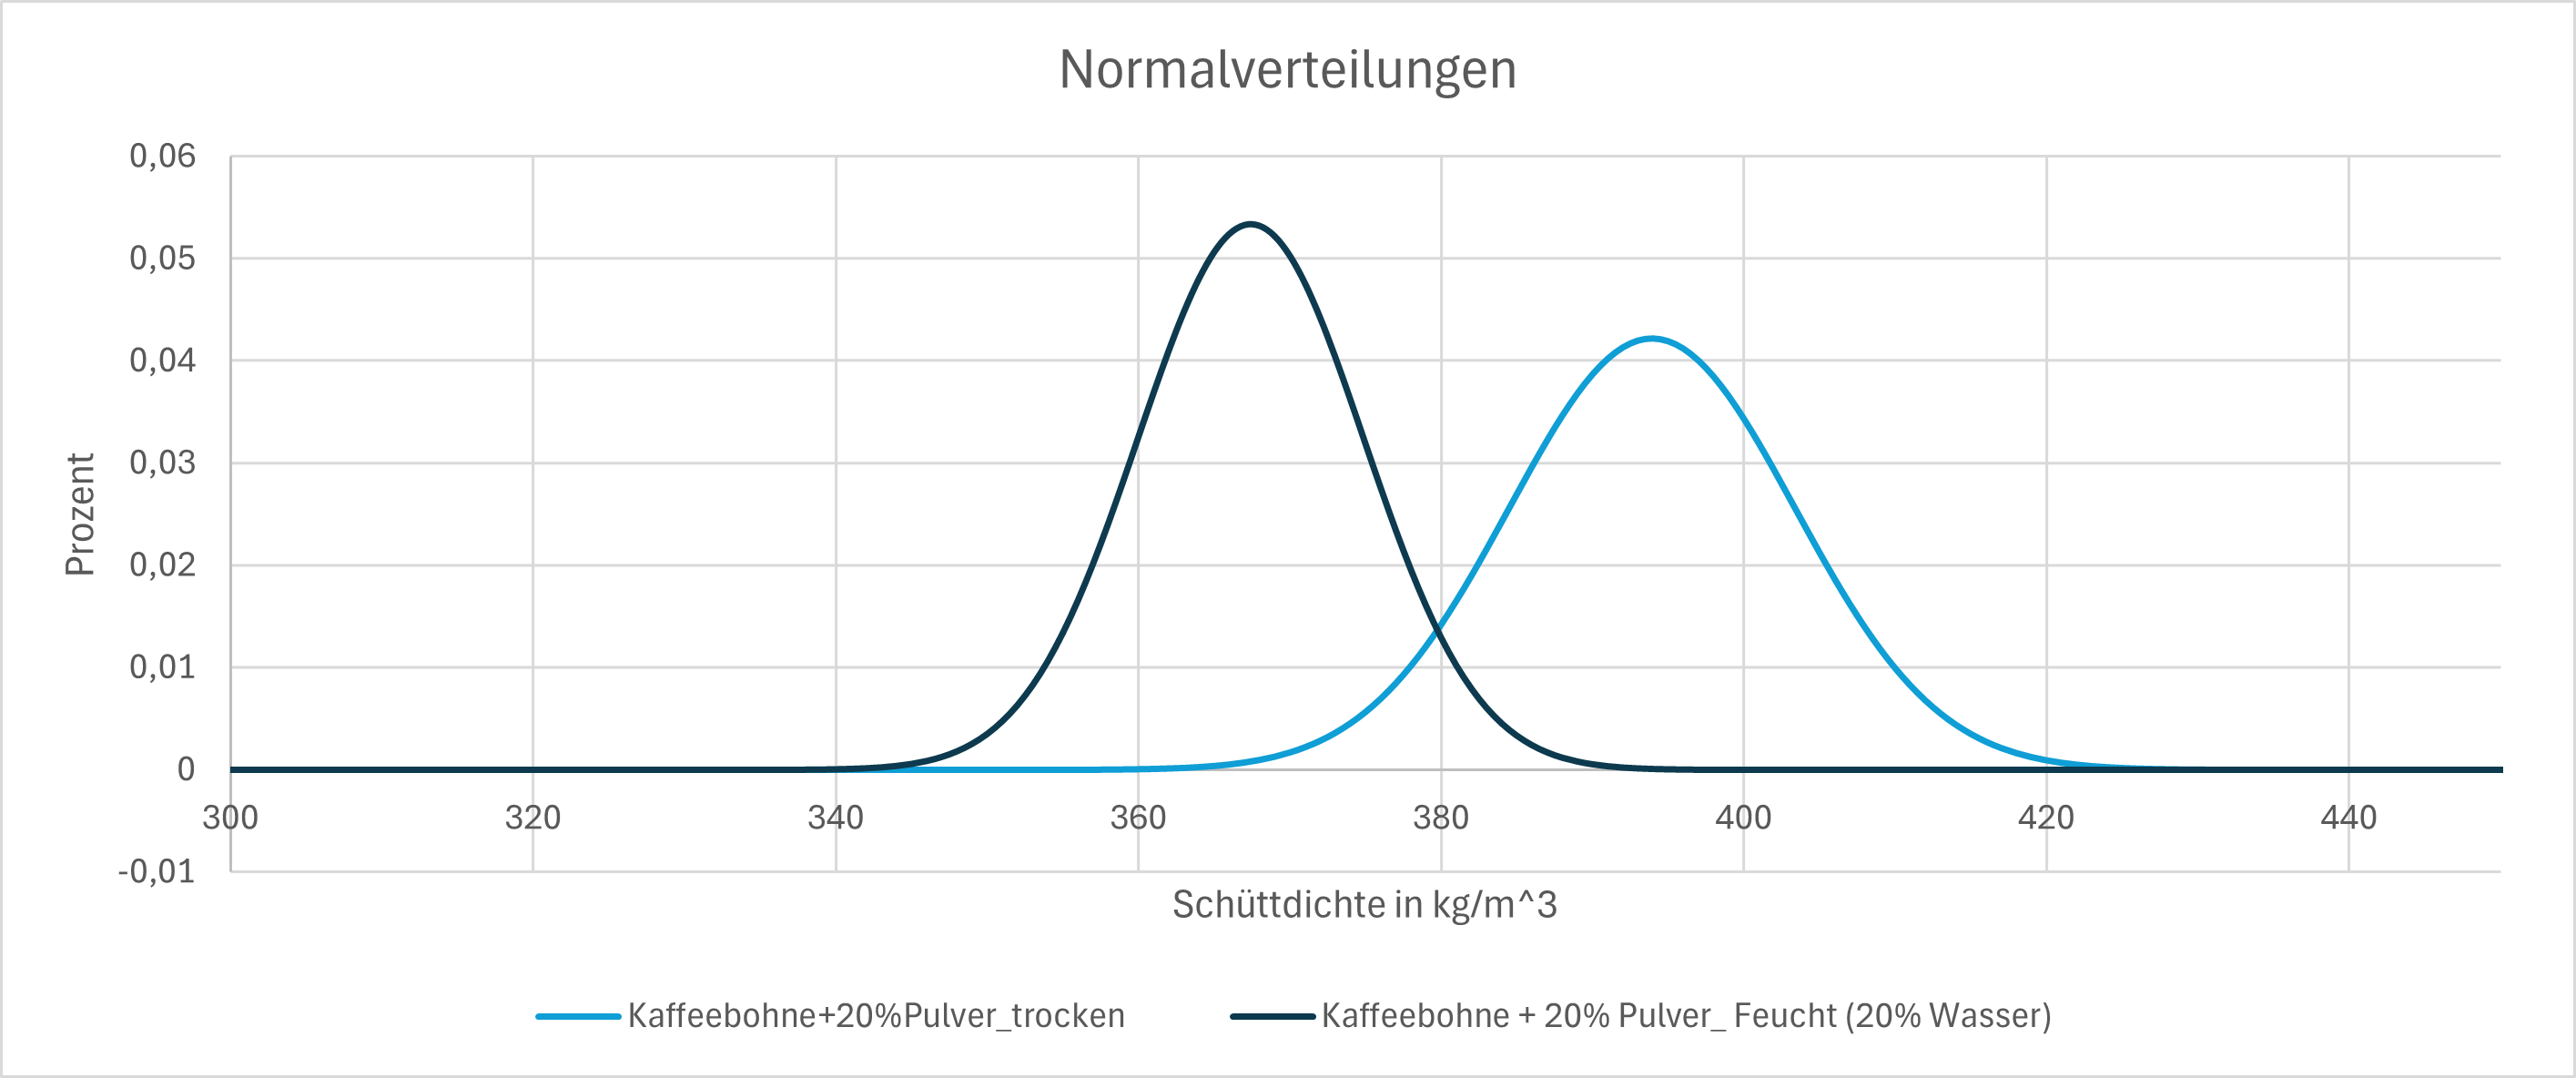
\includegraphics[width=0.8\textwidth]{Kaffeebohne-verunreinigung-trocken-vs-feucht.png}
        \caption{Normalverteilung Kaffeebohne-Verunreinigung-trocken-vs-feucht}
        \label{fig: Norm.Kaffeebohne-verunreinigung-trocken-vs-feucht}
    \end{figure}

    % Diagrammbeschreibung
    %---------------------
    In Abbildung \ref{fig: Norm.Kaffeebohne-verunreinigung-trocken-vs-feucht} ist der Einfluss
    von Feuchtigkeit auf die Schüttdichte bei verunreinigten Kaffeebohnen abgebildet. Obwohl die
    Schüttdichte bei den trockenen, verunreinigten Kaffeebohnen höher ist als bei den feuchten,
    lässt sich nicht mit Sicherheit sagen, dass es sich um ein signifikantes Ergebnis handelt.
    Um eine sichere Aussage zu treffen, müssten hier noch weitere Versuche durchgeführt werden.
    Würden diese Versuche zu besser separierten Verteilungen führen, könnte von einem
    signifikanten Einfluss gesprochen werden.
%==============================================================================================

\section{Verunreinigtes Kaffeepulver trocken vs feucht}
    % Bild Kaffeebohne trocken -Kaffeepulver trocken
    %-----------------------------------------------
    \begin{figure}[H]
        \centering
        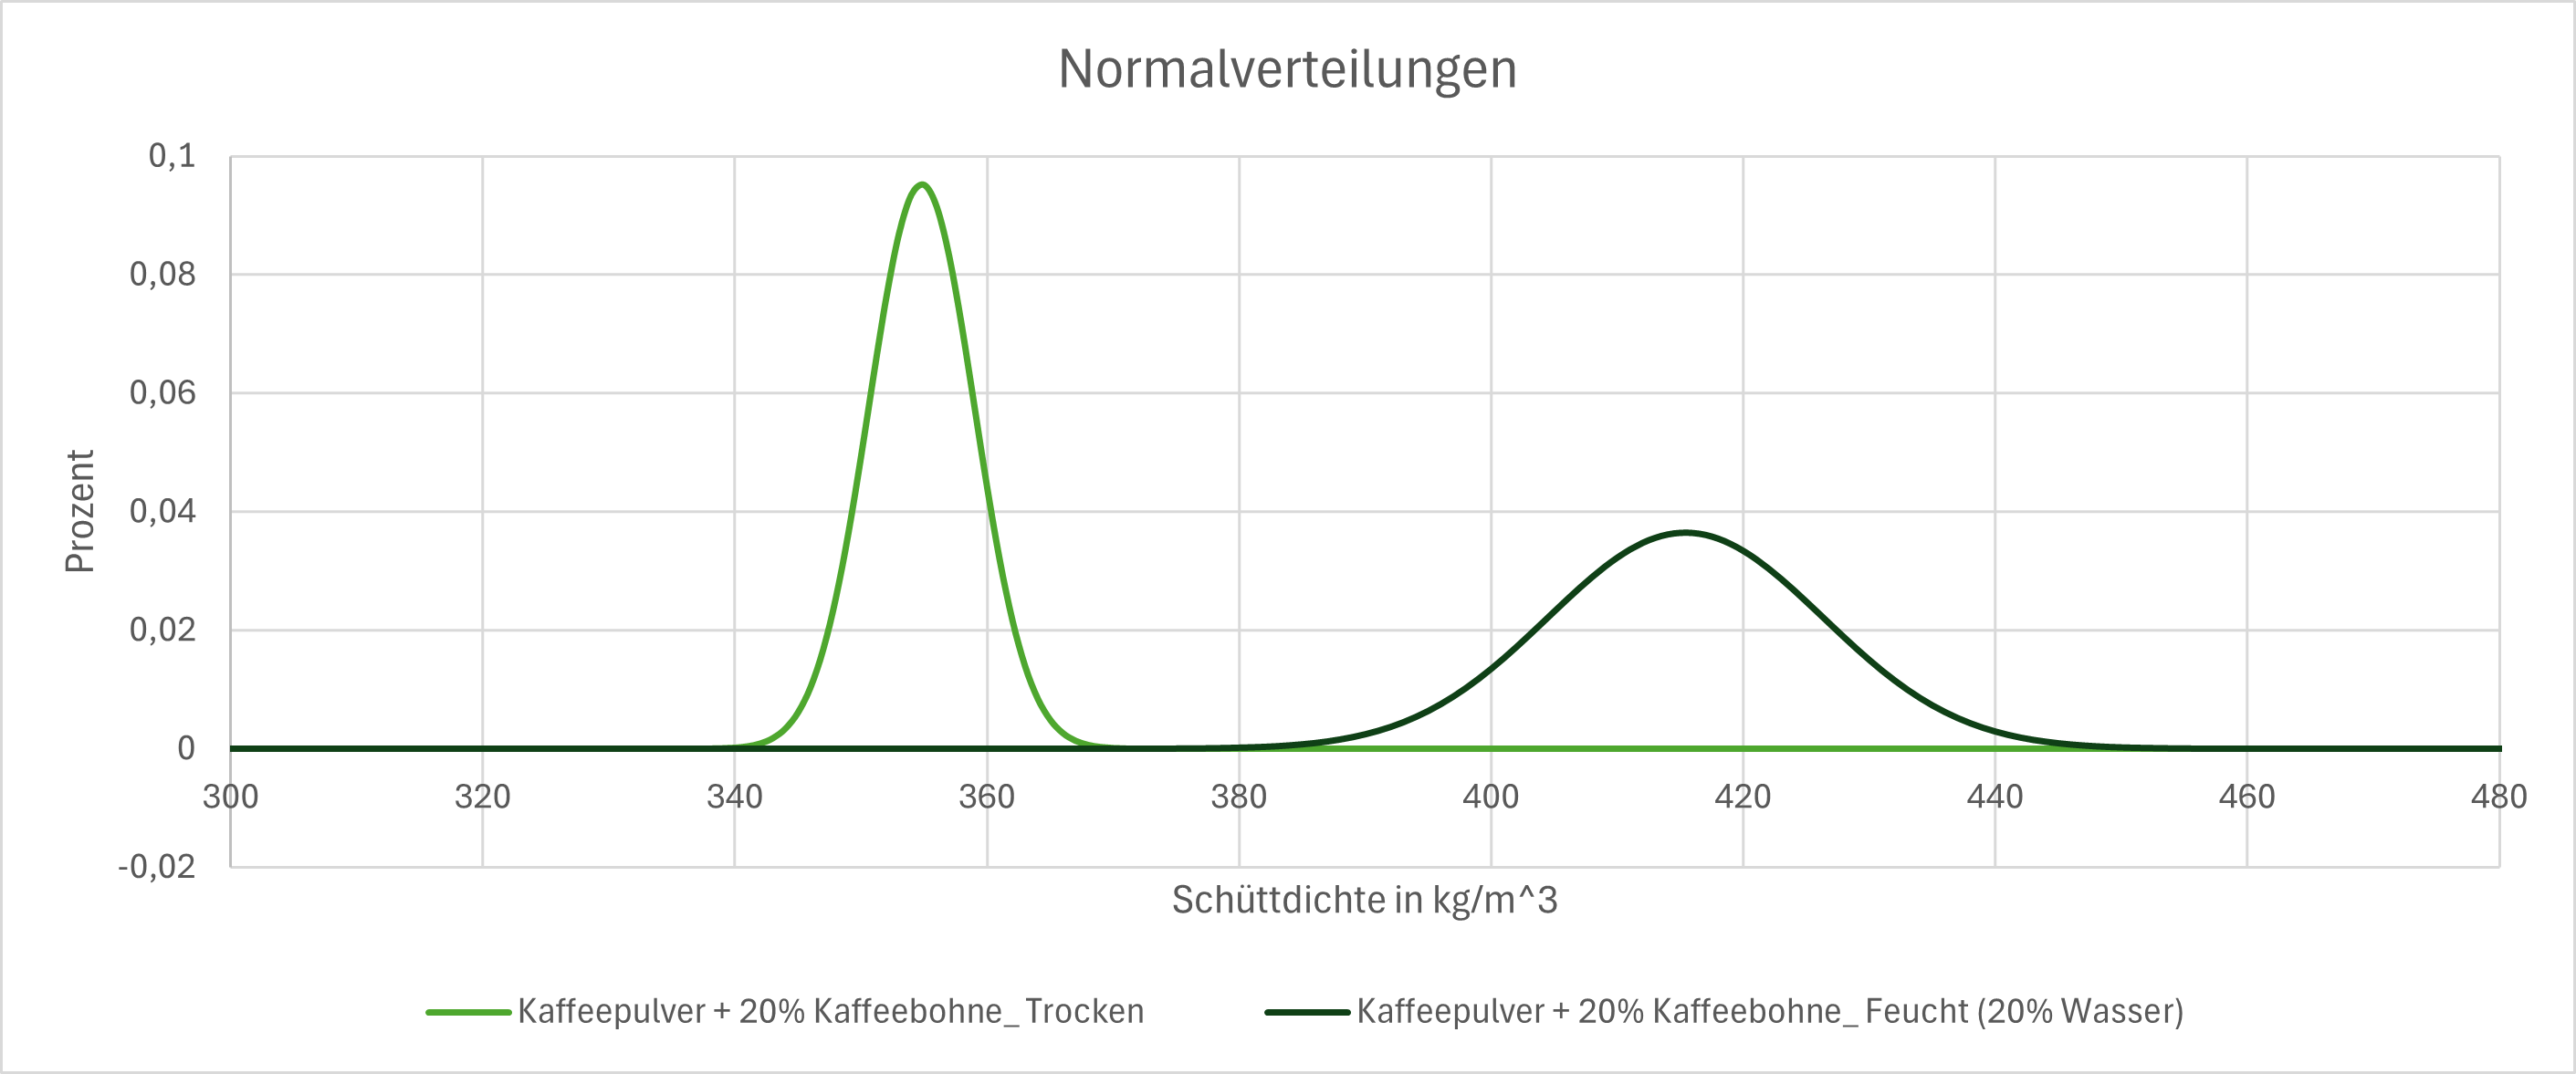
\includegraphics[width=0.8\textwidth]{Kaffeepulver-verunreinigung-trocken-vs-feucht.png}
        \caption{Normalverteilung Kaffeepulver-Verunreinigung-trocken-vs-feucht}
        \label{fig: Norm.Kaffeepulver-verunreinigung-trocken-vs-feucht}
    \end{figure}

    % Diagrammbeschreibung
    %---------------------
    In Abbildung \ref{fig: Norm.Kaffeepulver-verunreinigung-trocken-vs-feucht} ist der
    Einfluss der Feuchtigkeit auf Schüttdichte bei verunreinigtem Kaffepulver dargestellt. Es
    ist gut zu erkennen, dass die Schüttdichte von verunreinigtem Kaffepulver deutlich höher
    ist, wenn das Schüttgut Feuchte enthält. Der Einfluss von Feuchte kann aufgrund der
    beiden Verteilungen, die gut separiert sind, als hochsignifikant eingestuft werden.
%==============================================================================================

\section{Kaffeebohne feucht vs Verunreinigung Kaffeebohne feucht}
    % Bild Kaffeebohne trocken -Kaffeepulver trocken
    %-----------------------------------------------
    \begin{figure}[H]
        \centering
        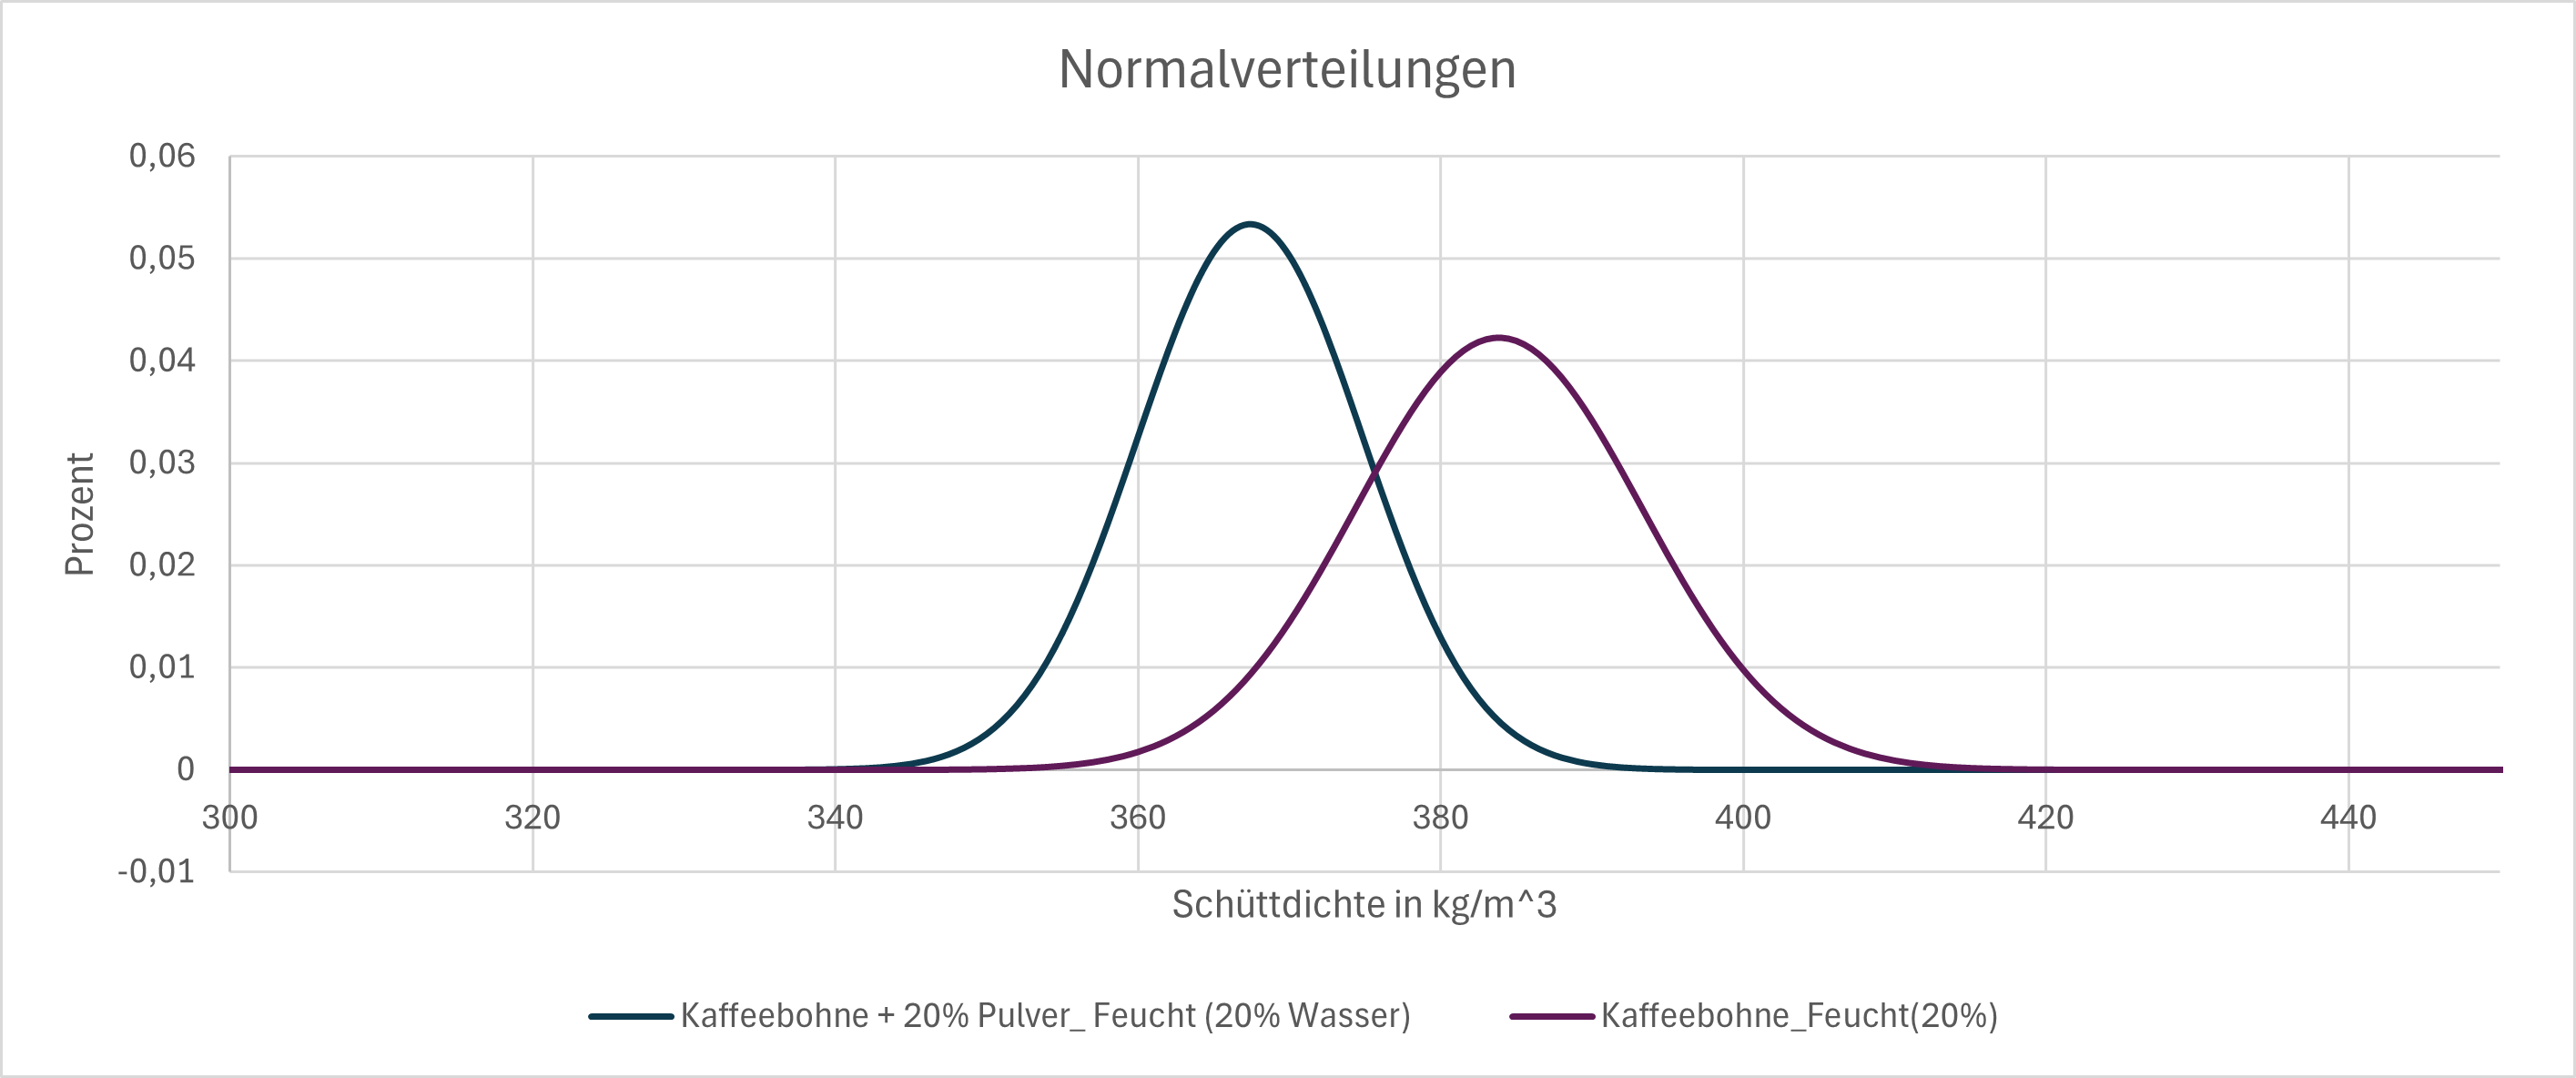
\includegraphics[width=0.8\textwidth]{Kaffeebohne_feucht-vs-Verunreinigung_Kaffeebohne_feucht.png}
        \caption{Normalverteilung Kaffeebohne feucht vs Verunreinigung Kaffeebohne feucht}
        \label{fig: Norm.Kaffeebohne_feucht-vs-Verunreinigung_Kaffeebohne_feucht}
    \end{figure}

    % Diagrammbeschreibung
    %---------------------
    In Abbildung \ref{fig: Norm.Kaffeebohne_feucht-vs-Verunreinigung_Kaffeebohne_feucht} wird
    der Einfluss von Verunreinigung auf die Schüttdichte bei feuchten Kaffeebohnen dargestellt.
    Wie im Diagramm ersichtlich, lässt sich kein signifikanter Einfluss der Verunreinigung
    erkennen. Somit kann angenommen werden, dass die Verunreinigung kaum Einfluss auf die
    Schüttdichte feuchter Bohnen hat.
%==============================================================================================

\section{Kaffeepulver feucht vs Verunreinigung Kaffeepulver feucht}
 % Bild Kaffeebohne trocken -Kaffeepulver trocken
 \begin{figure}[H]
    \centering
    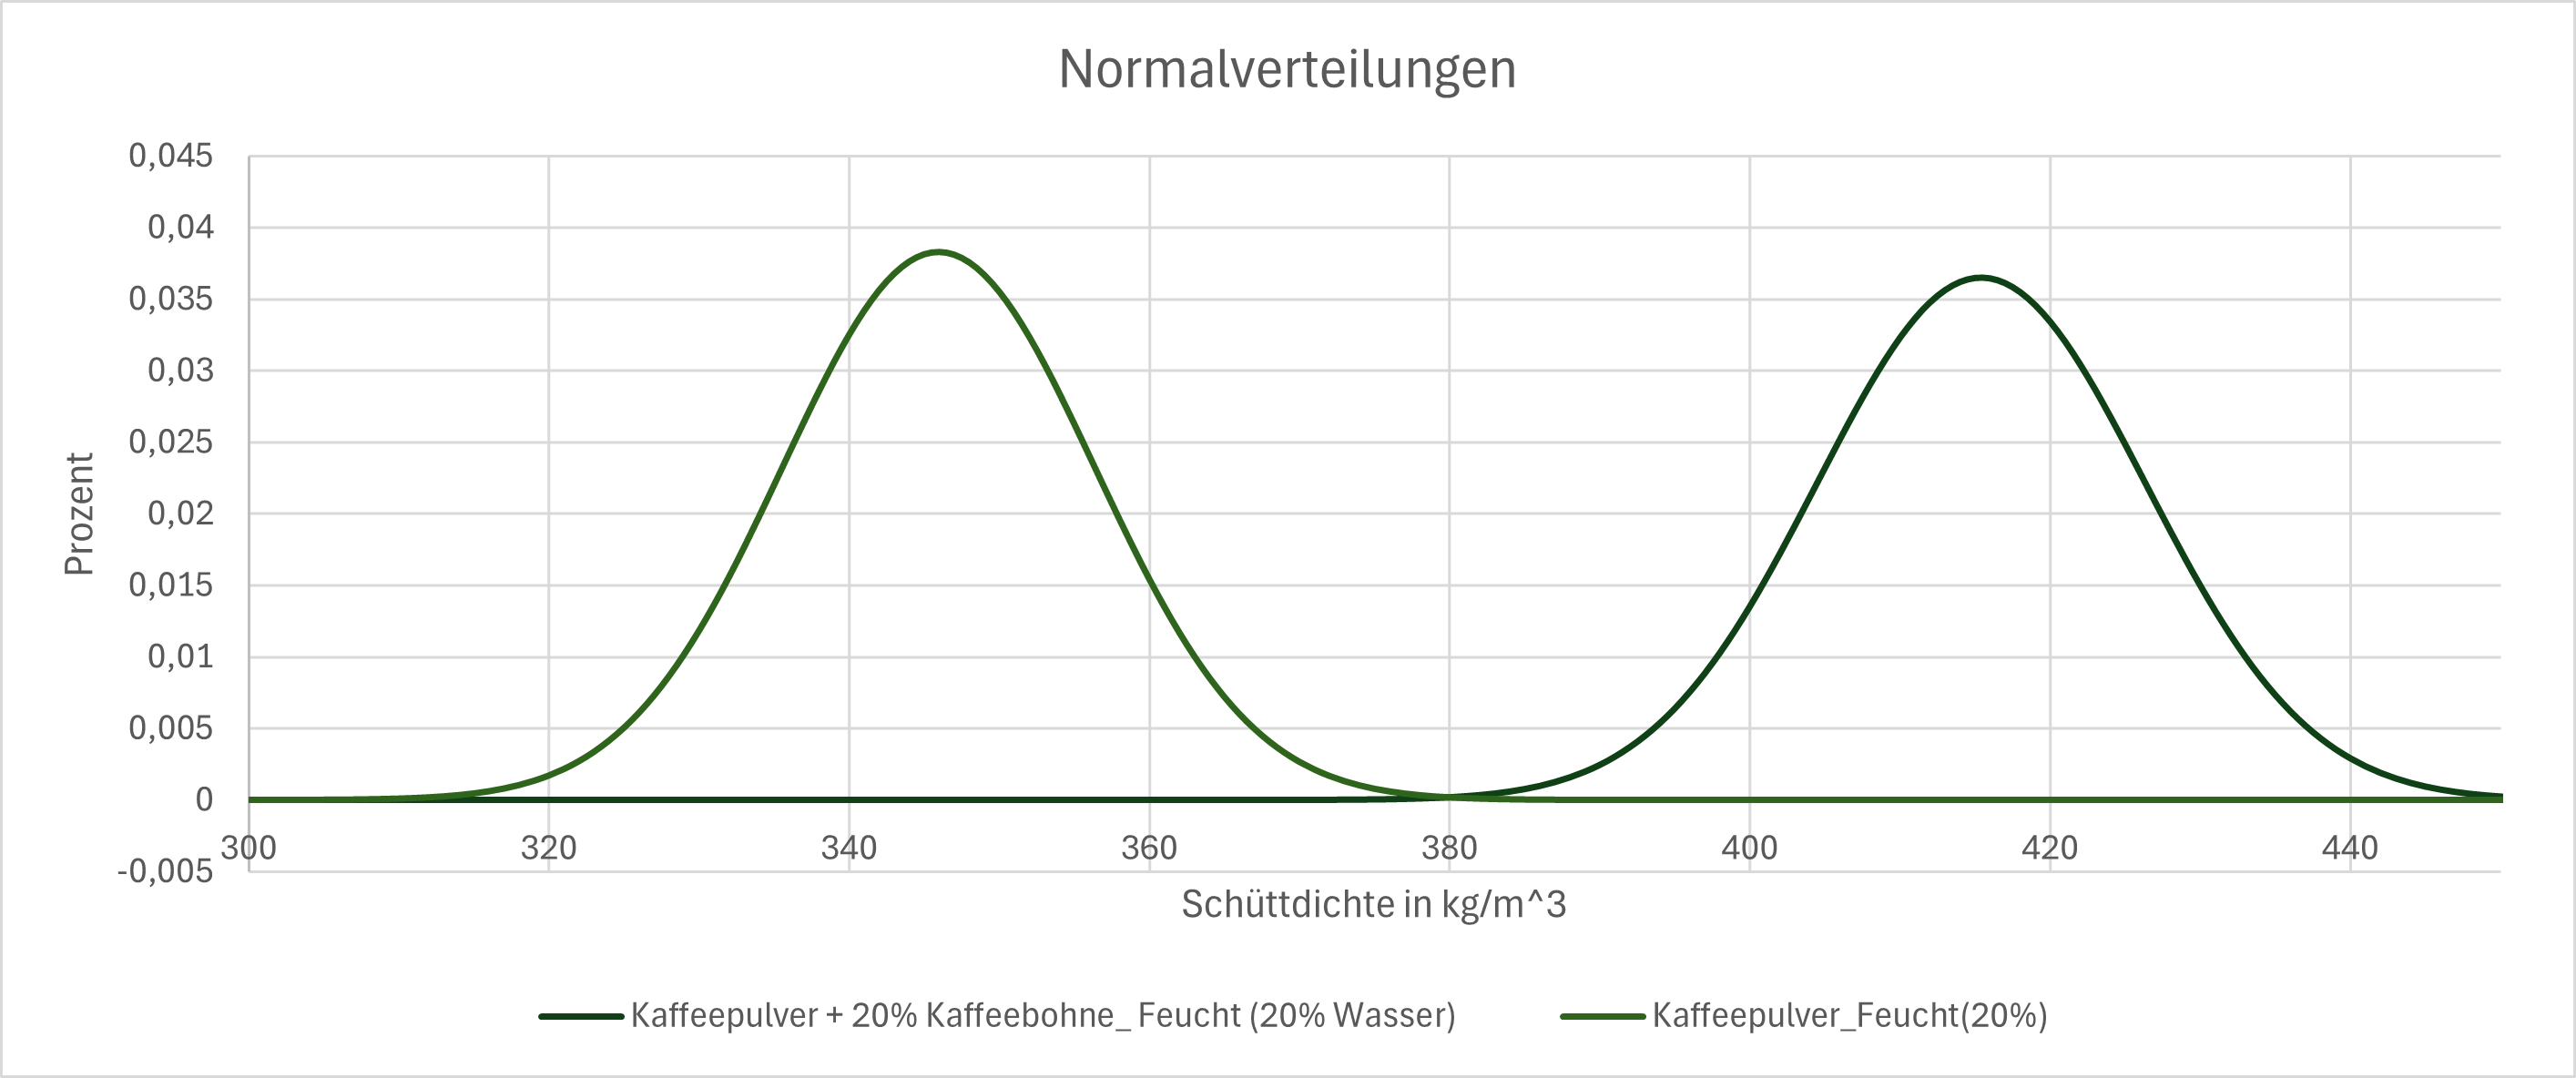
\includegraphics[width=0.8\textwidth]{Kaffeepulver_feucht-vs-Verunreinigung_Kaffeepulver_feucht.png}
    \caption{Normalverteilung Kaffeepulver feucht vs Verunreinigung Kaffeepulver feucht}
    \label{fig: Norm.Kaffeepulver_feucht-vs-Verunreinigung_Kaffeepulver_feucht}
\end{figure}

In Abbildung \ref{fig: Norm.Kaffeepulver_feucht-vs-Verunreinigung_Kaffeepulver_feucht} werden die Normalverteilungen von feuchtem
Kaffeepulver und von feuchtem, verunreinigten Kaffeepulver gegenüber gestellt. Es ist erkennbar, dass das verunreinigte Kaffeepulver
eine signifikant höhere Schüttgutdichte aufweist als das nicht verunreinigte Kaffeepulver.
%==============================================================================================

\section{Verunreinigung Kaffeebohne feucht vs Verunreinigung Kaffepulver feucht}
 % Bild Kaffeebohne trocken -Kaffeepulver trocken
 \begin{figure}[H]
    \centering
    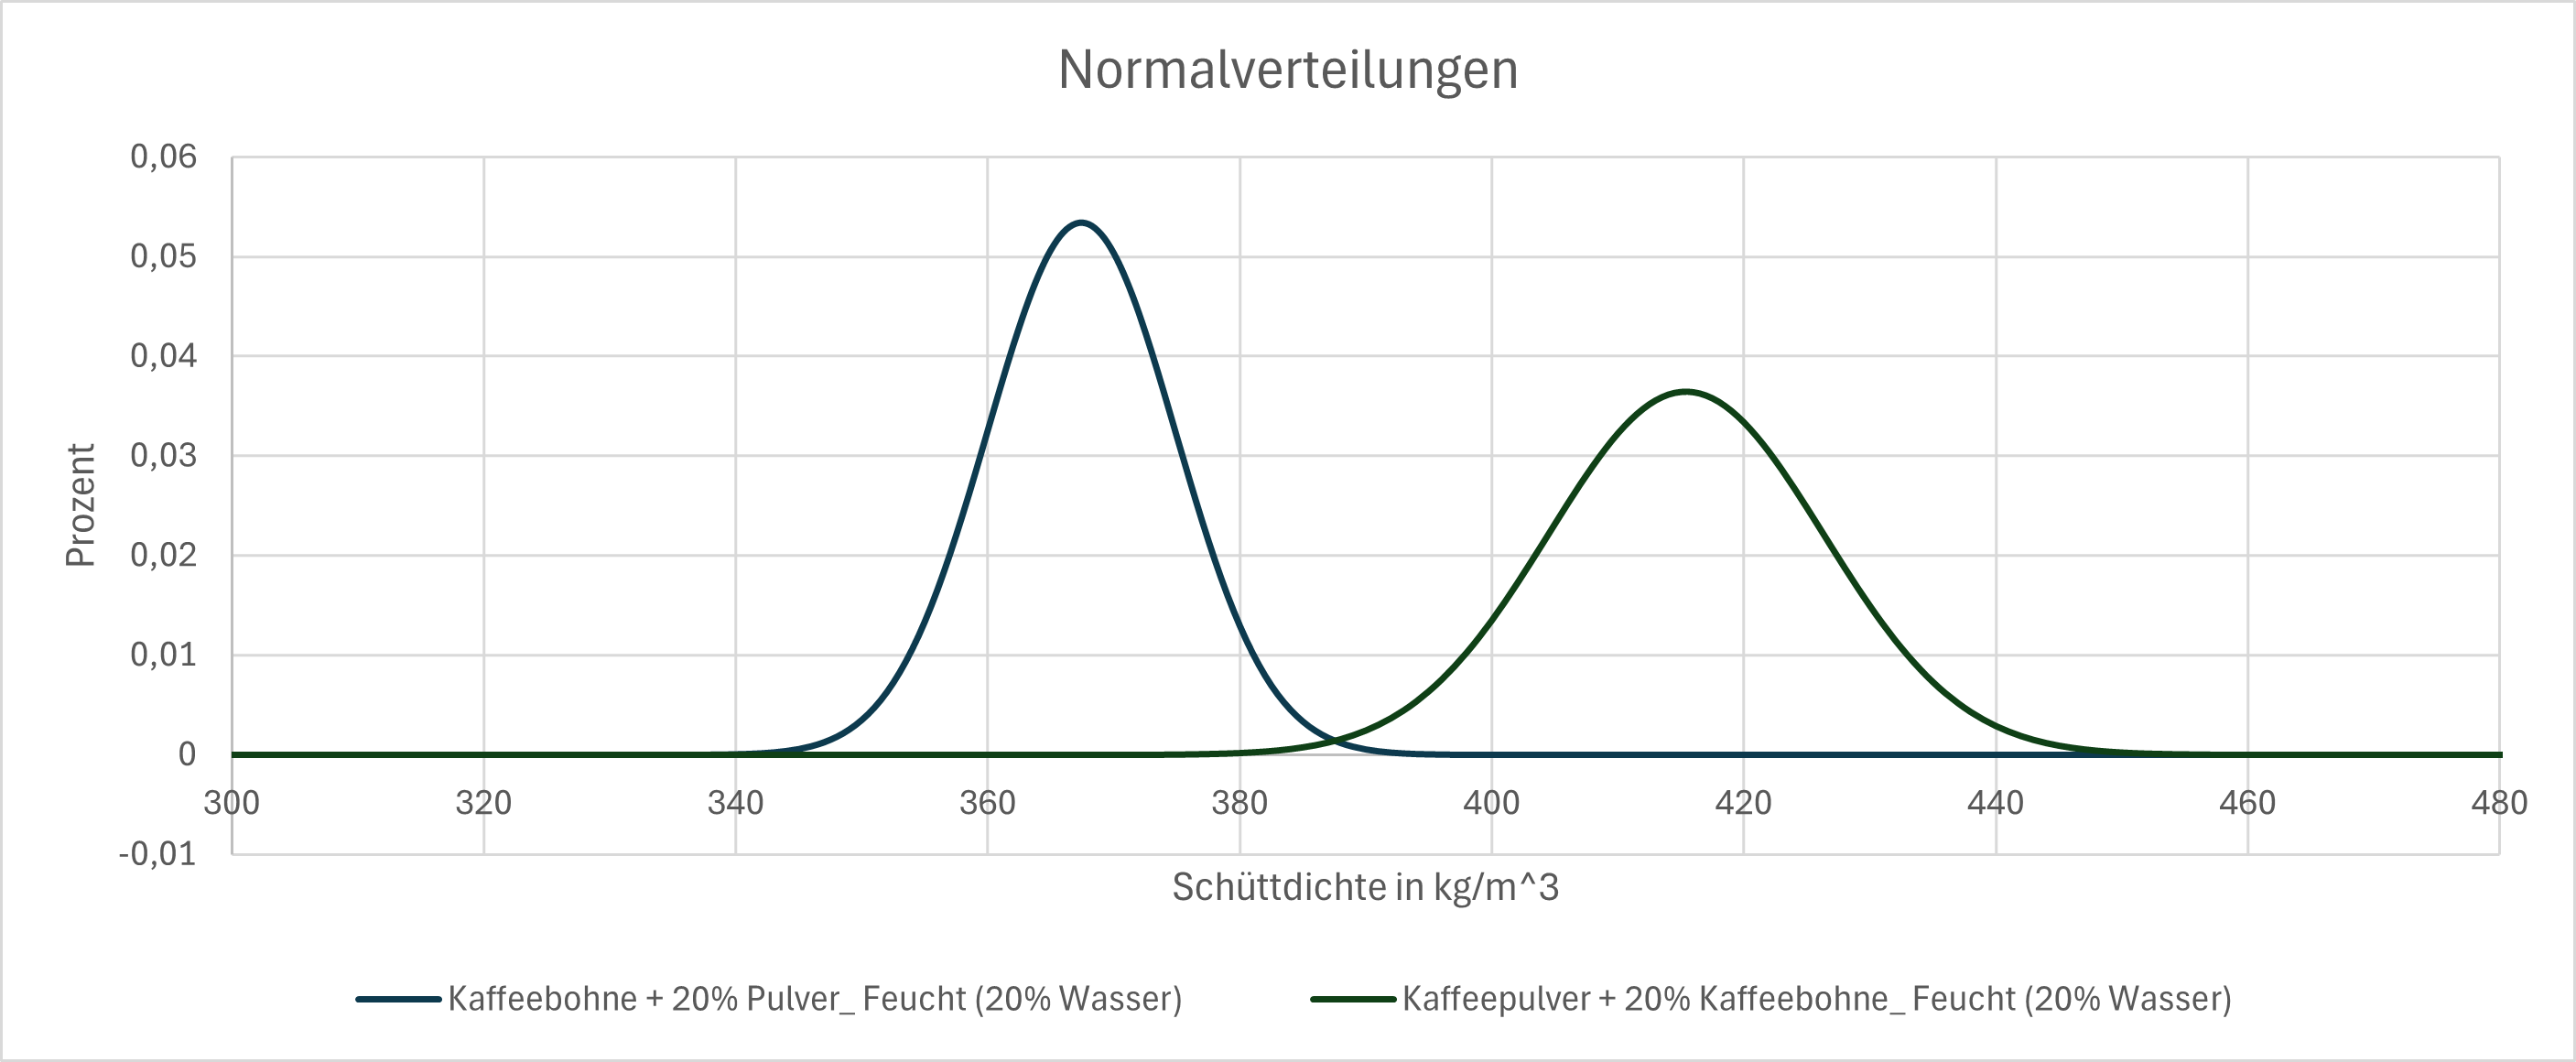
\includegraphics[width=0.8\textwidth]{Verunreinigung-feucht.png}
    \caption{Normalverteilung Verunreinigung-feucht}
    \label{fig: Norm.Verunreinigung-feucht}
\end{figure}

In Abbildung \ref{fig: Norm.Verunreinigung-feucht} wird die feuchte, verunreinigte Kaffeebohne mit dem feuchten, verunreinigten
Kaffeepulver verglichen. Der Feuchtigkeitsgrad sowie der Verunreinigungsgrad liegen bei Bohne und Pulver bei jeweils $20\%$.
Es lässt sich deutlich erkennen, dass das verunreinigte Pulver eine signifikant höhere Schüttdichte aufweist als die verunreinigte
Bohne.
%==============================================================================================

% Vollfaktorieller Versuchsplan
%==============================
\section{Vollfaktorieller Versuchsplan}
    % Einleitung
    %-----------
    Anhand der bisher erstellten Diagramme lassen sich keine eindeutigen Aussagen  bezüglich der
    Signifikanz von Effekten und Wechselwirkungen treffen. Daher wird die Auswertung nun anhand eines
    vollfaktoriellen Versuchsplans durchgeführt. Dieser ist in Abbildung
    \ref{fig: Vollfaktorieller_Versuchsplan} dargestellt. Die Werte der Einflussgrößen wurden dabei
    auf ein Intervall von -1 bis 1 normiert. -1 stellt die untere Stufe dar:

    \begin{itemize}
        \item kleine Korngröße $\rightarrow$ Kaffepulver
        \item 0 \% Feuchtigkeit
        \item 0 \% Verunreinigung 
    \end{itemize}

    % Bild - vollfaktorieller Versuchsplan
    %-------------------------------------
    \begin{figure}[H]
        \centering
        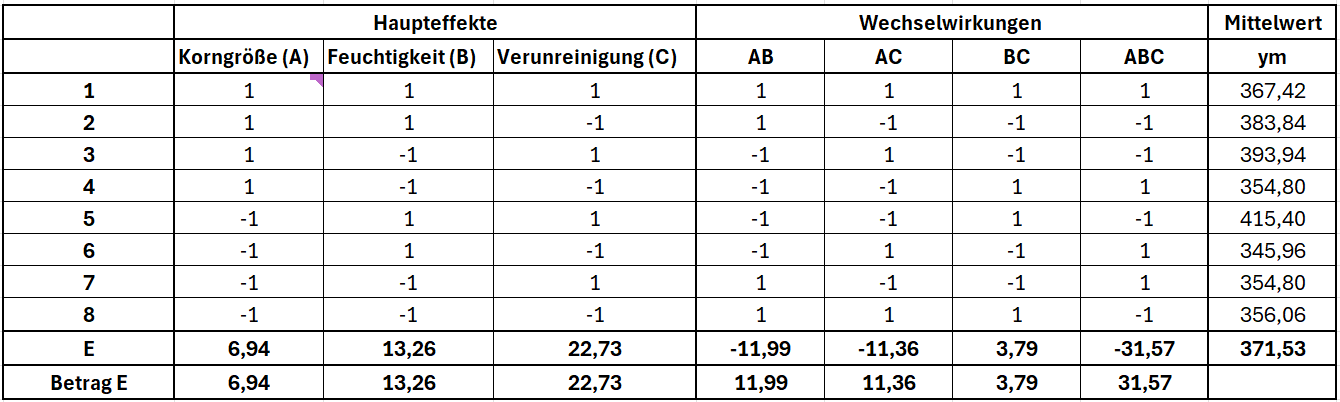
\includegraphics[width=1\textwidth]{Vollfaktorieller_Versuchsplan.png}
        \caption{Vollfaktorieller Versuchsplan}
        \label{fig: Vollfaktorieller_Versuchsplan}
    \end{figure}
    %------------------------------------------------------------------------------------------------

    % Diagrammbeschreibung
    %---------------------
    \noindent
    In Abbildung \ref{fig: Signififkanzniveau} wird dargestellt, wie signifikant die Haupteffekte und
    Wechselwirkungen sind. Dabei wird für jeden Haupteffekt / jede Wechselwirkung der Betrag mit
    einem Balken dargestellt. Außerdem werden die Vertrauensbereiche mit waagrechten Linien
    angezeigt. Die unterste, waagrechte Linie steht dabei für einen Vertrauensbereich von 95 \%, die
    mittlere für 99 \% und die oberste für 99,9 \%. Je nachdem, in welchem Bereich ein Balken endet,
    kann somit die Signifikanz des Haupteffekts / der Wechselwirkung abgelesen werden.

    % Bild - Signifikanzniveau
    %-------------------------
    \begin{figure}[H]
        \centering
        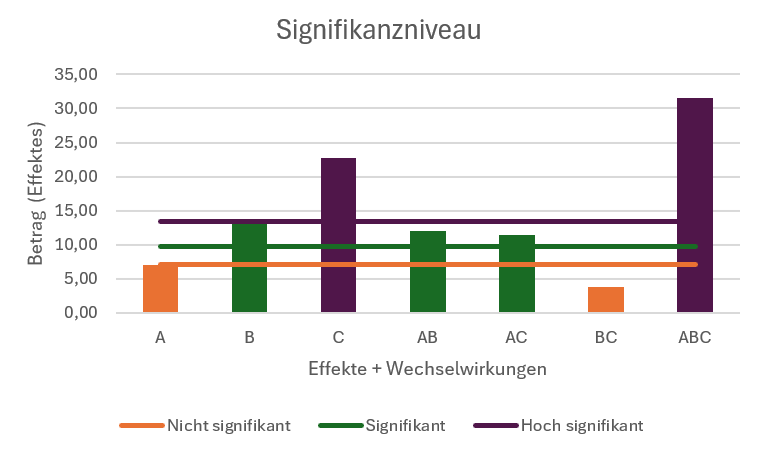
\includegraphics[width=0.8\textwidth]{Signififkanzniveau.png}
        \caption{Signififkanzniveau}
        \label{fig: Signififkanzniveau}
    \end{figure}

    % Interpretation des Diagramms
    %-----------------------------
    % hochsignifikant
    \noindent
    Aus Abbildung \ref{fig: Signififkanzniveau} geht hervor, dass die die Verunreinigung sich
    hochsignifikant auf die Packungsdichte auswirkt. Außerdem liegt eine hochsignifikante 3-fach
    Wechselwirkung zwischen Korngröße, Feuchtigkeit und Verunreinigung vor.
    \\

    % signifikant
    \noindent
    Weiters ist zu sehen, dass die Feuchtigkeit einen signifikanten Einfluss auf die Packungsdichte
    hat. Auch die Wechselwirkungen zwischen Korngröße und Feuchtigkeit und zwischen Korngröße und
    Verunreinigung sind signifikant. Es muss allerdings erwähnt werden, dass der Einfluss der
    Feuchtigkeit nur knapp unterhalb der Grenze zum hochsignifikanten Einfluss liegt. Um also mit
    Sicherheit sagen zu können, dass es sich nur um einen signifikanten Einfluss handelt, müssten noch
    mehr Versuche durchgeführt werden.
    \\

    % nicht signifikant
    \noindent
    Als nicht signifikanter Einflussfaktor hat sich die Korngröße herausgestellt. Allderings
    liegt auch der Einfluss der Korngröße nur knapp unter der Grenze zum signifikanten
    Einfluss. Demnach müssten auch bei der Korngröße weitere Versuche gemacht werden.
    Die Wechselwirkung zwischen Feuchtigkeit und Verunreinigung ist dagegen deutlich nicht
    signifikant.